\chapter{Universal Serial Bus}

This chapter presents an overview of the \textit{Universal Serial Bus} (USB) \textit{Full Speed} interface, with focus on the features used in the GEX firmware. USB is a versatile but complex interface, thus explaining it in its entirety is beyond the scope of this text. References to external materials which explain the protocol in greater detail will be provided for the interested reader.\todo{add those refs}

\section{Basic Principles and Terminology}

\todo[inline]{add a diagram of the hierarchical topology}

USB is a hierarchical bus with a single master (\textit{host}) and multiple slave devices. A USB device that provides functionality to the host is called a \textit{function}. Communication between the host and a function is organized into virtual channels called \textit{pipes}. Each pipe is identified by an \textit{endpoint} number. 

Endpoints can be either unidirectional or bidirectional; the direction from the host to a function is called \textit{OUT}, the other direction (function the host) is called IN. A bidirectional endpoint is technically composed of a IN and OUT endpoint with the same number. All transactions (both IN and OUT) are initiated by the host; functions have to wait for their turn. Endpoint 0 is bidirectional, always enabled, and serves as a \textit{control endpoint}. The host uses the control endpoint to read information about the device and configure it as needed.

There are four types of transfers: control, bulk, isochronous, and interrupt. Each endpoint is configured for a fixed transfer type. 

\begin{itemize}
	\item \textit{Control} - initial configuration after device plug-in; also used for other aplication-specific control messages that can affect other pipes.
	\item \textit{Bulk} - used for burst transfers of large messages, commonly e.g. for mass storage devices
	\item \textit{Isochronous} - streaming with guaranteed low latency; designed for audio or video streams where some data loss is preferred over stuttering
	\item \textit{Interrupt} - low latency short messages, used for human interface devices like mice and keyboards
\end{itemize}

The endpoint transfer type and other characteristics, together with other information about the device, such as the serial number, are defined in a \textit{descriptor table}. This is a tree-like binary structure defined in the function's memory. The descriptor table is loaded by the host to learn about the used endpoints and to attach the right driver to it.

The function's endpoints are grouped into \textit{interfaces}. An interface describes a logical connection of endpoints, such as the reception and transmission endpoint that belong together. An interface is assigned a \textit{class} defining how it should be used. Standard classes are defined by the USB specification to provide a uniform way of interfacing devices of the same type, such as human-interface devices (mice, keyboards, gamepads) or mass storage devices. The use of standard classes makes it possible to re-use the same driver software for devices from different manufacturers. The class used for the GEX's "virtual COM port" function was originally meant for telephone modems, a common way of connecting to the Internet at the time the first versions of USB were developed. A device using this class will show as \verb|/dev/ttyACM0| on Linux and as a COM port on Windows, provided the system supports it natively or the right driver is installed.

\todo[inline]{add reference to the document}

\todo[inline]{fix: massive gap here}

\todo[inline]{function - https://technet.microsoft.com/en-us/library/cc939102.aspx}

\newpage
\hspace*{-1.5em}
\begin{minipage}[t]{0.5\textwidth}\scriptsize
\begin{verbatim}
Device Descriptor:
  bLength                18
  bDescriptorType         1
  bcdUSB               2.00
  bDeviceClass          239 Miscellaneous Device
  bDeviceSubClass         2 
  bDeviceProtocol         1 Interface Association
  bMaxPacketSize0        64
  idVendor           0x0483 STMicroelectronics
  idProduct          0x572a 
  bcdDevice            0.01
  iManufacturer           1 MightyPork
  iProduct                2 GEX
  iSerial                 3 0029002F-42365711-32353530
  bNumConfigurations      1
  Configuration Descriptor:
    bLength                 9
    bDescriptorType         2
    wTotalLength           98
    bNumInterfaces          3
    bConfigurationValue     1
    iConfiguration          0 
    bmAttributes         0x80
      (Bus Powered)
    MaxPower              500mA
    Interface Descriptor:
      bLength                 9
      bDescriptorType         4
      bInterfaceNumber        0
      bAlternateSetting       0
      bNumEndpoints           2
      bInterfaceClass         8 Mass Storage
      bInterfaceSubClass      6 SCSI
      bInterfaceProtocol     80 Bulk-Only
      iInterface              4 Settings VFS
      Endpoint Descriptor:
        bLength                 7
        bDescriptorType         5
        bEndpointAddress     0x81  EP 1 IN
        bmAttributes            2
          Transfer Type            Bulk
          Synch Type               None
          Usage Type               Data
        wMaxPacketSize     0x0040  1x 64 bytes
        bInterval               0
      Endpoint Descriptor:
        bLength                 7
        bDescriptorType         5
        bEndpointAddress     0x01  EP 1 OUT
        bmAttributes            2
          Transfer Type            Bulk
          Synch Type               None
          Usage Type               Data
        wMaxPacketSize     0x0040  1x 64 bytes
        bInterval               0
    Interface Association:
      bLength                 8
      bDescriptorType        11
      bFirstInterface         1
      bInterfaceCount         2
      bFunctionClass          2 Communications
      bFunctionSubClass       2 Abstract (modem)
      bFunctionProtocol       1 AT-commands (v.25ter)
      iFunction               5 Virtual Comport ACM
\end{verbatim}
\end{minipage}\hspace{1em}
\begin{minipage}[t]{0.5\textwidth}\scriptsize
\begin{verbatim}
    Interface Descriptor:
      bLength                 9
      bDescriptorType         4
      bInterfaceNumber        1
      bAlternateSetting       0
      bNumEndpoints           1
      bInterfaceClass         2 Communications
      bInterfaceSubClass      2 Abstract (modem)
      bInterfaceProtocol      1 AT-commands (v.25ter)
      iInterface              5 Virtual Comport ACM
      CDC Header:
        bcdCDC               1.10
      CDC Call Management:
        bmCapabilities       0x00
        bDataInterface          2
      CDC ACM:
        bmCapabilities       0x06
          sends break
          line coding and serial state
      CDC Union:
        bMasterInterface        1
        bSlaveInterface         2 
      Endpoint Descriptor:
        bLength                 7
        bDescriptorType         5
        bEndpointAddress     0x83  EP 3 IN
        bmAttributes            3
          Transfer Type            Interrupt
          Synch Type               None
          Usage Type               Data
        wMaxPacketSize     0x0008  1x 8 bytes
        bInterval             255
    Interface Descriptor:
      bLength                 9
      bDescriptorType         4
      bInterfaceNumber        2
      bAlternateSetting       0
      bNumEndpoints           2
      bInterfaceClass        10 CDC Data
      bInterfaceSubClass      0 
      bInterfaceProtocol      0 
      iInterface              6 Virtual Comport CDC
      Endpoint Descriptor:
        bLength                 7
        bDescriptorType         5
        bEndpointAddress     0x02  EP 2 OUT
        bmAttributes            2
          Transfer Type            Bulk
          Synch Type               None
          Usage Type               Data
        wMaxPacketSize     0x0040  1x 64 bytes
        bInterval               0
      Endpoint Descriptor:
        bLength                 7
        bDescriptorType         5
        bEndpointAddress     0x82  EP 2 IN
        bmAttributes            2
          Transfer Type            Bulk
          Synch Type               None
          Usage Type               Data
        wMaxPacketSize     0x0040  1x 64 bytes
        bInterval               0
\end{verbatim}
\end{minipage}\vspace{-1em}
\begin{figure}[H]
	\cprotect\caption{USB descriptors of a GEX prototype obtained using \verb|lsusb -vd vid:pid|}
\end{figure}


\section{USB Physical Layer}

USB uses differential signaling with NRZI encoding (\textit{Non Return to Zero Inverted}, fig. \ref{fig:nrzi}) and bit stuffing. The encoding, together with frame formatting, checksum verification, retransmission, and other low level aspects of the USB connection are entirely handled by the USB block in the microcontroller's silicon; normally we do not need to worry about those details. What needs more attention are the electrical characteristics of the bus, which need to be understood correctly for a successful schematic and PCB design.

\begin{wrapfigure}[4]{r}{0.4\textwidth}
	\centering
	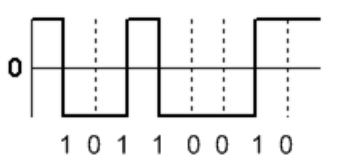
\includegraphics[width=0.3\textwidth]{img/usb-nrzi-diagram.png}
	\caption{\label{fig:nrzi}NRZI encoding example}
\end{wrapfigure}

The USB cable contains 4 conductors:

\begin{itemize}\setlength\itemsep{.2em}
	\item V$_\mathrm{BUS}$ (+5\,V)
	\item D+
	\item D--
	\item Ground
\end{itemize}

The data lines, D+ and D--, are also commonly labeled DP and DM. This differential pair should be routed in parallel and kept at approximately the same length.

USB revisions are, where possible, backwards compatible, often even keeping the same connector shape. The bus speed is negotiated by the device using a 1.5\,k$\Omega$ pull-up resistor to 3.3\,V on one of the data lines: for Full Speed, D+ is pulled high (fig. \label{fig:usb-pullup-fs}), for Low Speed it's on D--. The polarity of the differential signals is inverted depending on the used speed. Some microcontrollers integrate the correct pull-up resistor inside the USB block (including out STM32F072), removing the need for an external resistor.

\begin{figure}
	\centering
	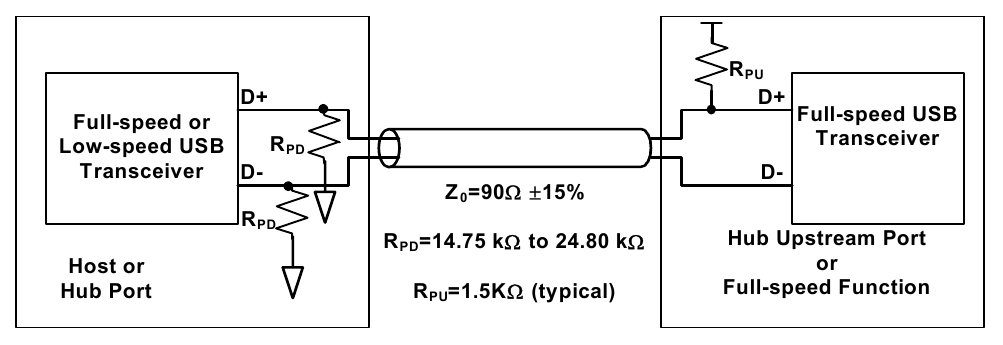
\includegraphics[width=\textwidth]{img/usb-pullup-fs.png}
	\caption{\label{fig:usb-pullup-fs}Pull-up and pull-down resistors of a Full Speed function, as prescribed by the USB specification rev. 2.0}
\end{figure}

When a function wants to be re-enumerated by the host, which is needed to reload the descriptors and re-attach the correct drivers, it can momentarily remove the pull-up resistor, which the host will interpret as if the device was plugged out. With an internal pull-up this can be done by flipping a bit in a control register. An external resistor can be connected through a transistor controlled by a GPIO pin. 

\todo[inline]{https://www.eevblog.com/forum/projects/driving-the-1k5-usb-pull-up-resistor-on-d/}
\todo[inline]{http://www.beyondlogic.org/usbnutshell/usb2.shtml}

The V$_\mathrm{BUS}$ line supplies power to \textit{bus-powered} devices. \textit{Self-powered} devices can leave this pin unconnected and instead use an external power supply. The maximal current drawn from the V$_\mathrm{BUS}$ line is configured using a descriptor and should not be exceeded, but experiments suggest this is often not enforced.

\section{USB Classes}

This section explains the Mass Storage class and the CDC/ACM class that are used in the GEX firmware. A list of all standard classes with a more detailed explanation can be found in \todo{link to the ref manual}.

\subsection{Mass Storage Class}

The Mass Storage class (MSC) is supported by all modern operating systems (MS Windows, MacOS, GNU/Linux, FreeBSD etc.) to support thumb drives, external disks, memory card readers and other storage devices.
\todo[inline]{links}
%http://www.usb.org/developers/docs/devclass_docs/Mass_Storage_Specification_Overview_v1.4_2-19-2010.pdf
%http://www.usb.org/developers/docs/devclass_docs/usbmassbulk_10.pdf

The MSC specification defines multiple \textit{transport protocols} that can be selected using the descriptors. For it's simplicity, the \textit{Bulk Only Transport} (BOT) will be used. BOT uses two bulk endpoints for reading and writing blocks of data and for the exchange of control commands and status messages. For the device to be recognized by the operating system, it must also implement a \textit{command set}. Most mass storage devices use the \textit{SCSI Transparent command set} 
\footnote{To confirm this assertion, the descriptors of five thumb drives and an external hard disk were analyzed using \verb|lsusb|. All but one device used the SCSI command set, one (the oldest thumb drive) used \textit{SFF-8070i}. A list of possible command sets can be found in TODO (usb spec overview)}.
The command set's commands let the host read information about the attached storage, such as its capacity, and check for media presence and readiness to write or detach. This is used e.g. for the "Safely Remove" function which checks that all internal buffers have been written to Flash.

\todo[inline]{links}

% weird flash - SFF-8070i subclass

% usb spec overview https://cscott.net/usb_dev/data/devclass/msco_v109.pdf

%https://bits4device.wordpress.com/2013/05/24/usb-mass-storage-class-msc-bulk-only-transfer-bot/

%http://janaxelson.com/mass_storage_faq.htm

The MSC class together with the SCSI command set are implemented in a USB Device library provided by ST Microelectronics. The library also includes a basic CDC/ACM implementation (see below).

In order to emulate a mass storage device without having a physical storage medium, we need to generate and parse the filesystem on-the-fly as the host OS tries to access it. This will be discussed in chapter ??\todo{chapter num}.

\subsection{CDC/ACM Class} \label{sec:cdc-acm}

%https://www.keil.com/pack/doc/mw/USB/html/group__usbd__cdc_functions__acm.html

Historically meant for modem communication, this class is now the de facto standard way of making USB devices appear as serial ports on the host OS. The CDC (\textit{Communication Device Class}) uses three endpoints: bulk IN and OUT, and an interrupt endpoint. 

\todo{verify this vvv}
The interrupt endpoint is used for control commands and notifications while the bulk endpoints are used for useful data. ACM stands for \textit{Abstract Control Model} and it's a CDC's subclass that defines the control messages format. Since we don't use a physical UART and the line is virtual both on the PC and in the end device, the control commands can be ignored.

An interesting property of this class is that the bulk endpoints transport raw data without any wrapping frames. By changing the device class in the descriptor table to 255 (\textit{Vendor Specific Class}), we can retain the messaging functionality of the designated endpoints and access the device directly using e.g. libUSB, while the OS will ignore it and won't try to attach any driver that could interfere otherwise. The same trick can be used to hide the mass storage class when not needed.

\subsection{Interface Association: Composite Class}

Since it's creation, the USB specification expected that each function will have only one interface enabled at a time. After it became apparent that there is a need for having multiple unrelated interfaces work in parallel, a workaround called the \textit{Interface Association Descriptor} (IAD) was introduced. IAD is an entry in the descriptor table that defines which interfaces belong together and should be handled by the same software driver.

To use the IAD, the function's class must be set to 239 (EFh), subclass 2 and protocol 1, so the OS knows to look for the presence of IADs before binding drivers to any interfaces. 

% TODO link to some references..

In GEX, the IAD is used to tie together the CDC and ACM interfaces while leaving out the MSC interface which should be handled by a different driver. To make this work, a new \textit{composite class} had to be created as a wrapper for the library-provided MSC and CDC/ACM implementations.

%http://www.usb.org/developers/docs/whitepapers/iadclasscode_r10.pdf




